\documentclass[review,12pt,number]{elsarticle}

\usepackage[T1]{fontenc}
\usepackage[utf8]{inputenc}
\usepackage{newtxtext}
\usepackage{newtxmath}
\usepackage{amsmath}
\usepackage{array}
\usepackage{booktabs}
\usepackage{graphicx}
\usepackage{hyperref}
\usepackage{lineno}
\usepackage{url}

\journal{Journal of Environmental Chemical Engineering}
\hypersetup{hidelinks}
\modulolinenumbers[5]
\setlength{\emergencystretch}{3em}

\begin{document}

\begin{graphicalabstract}
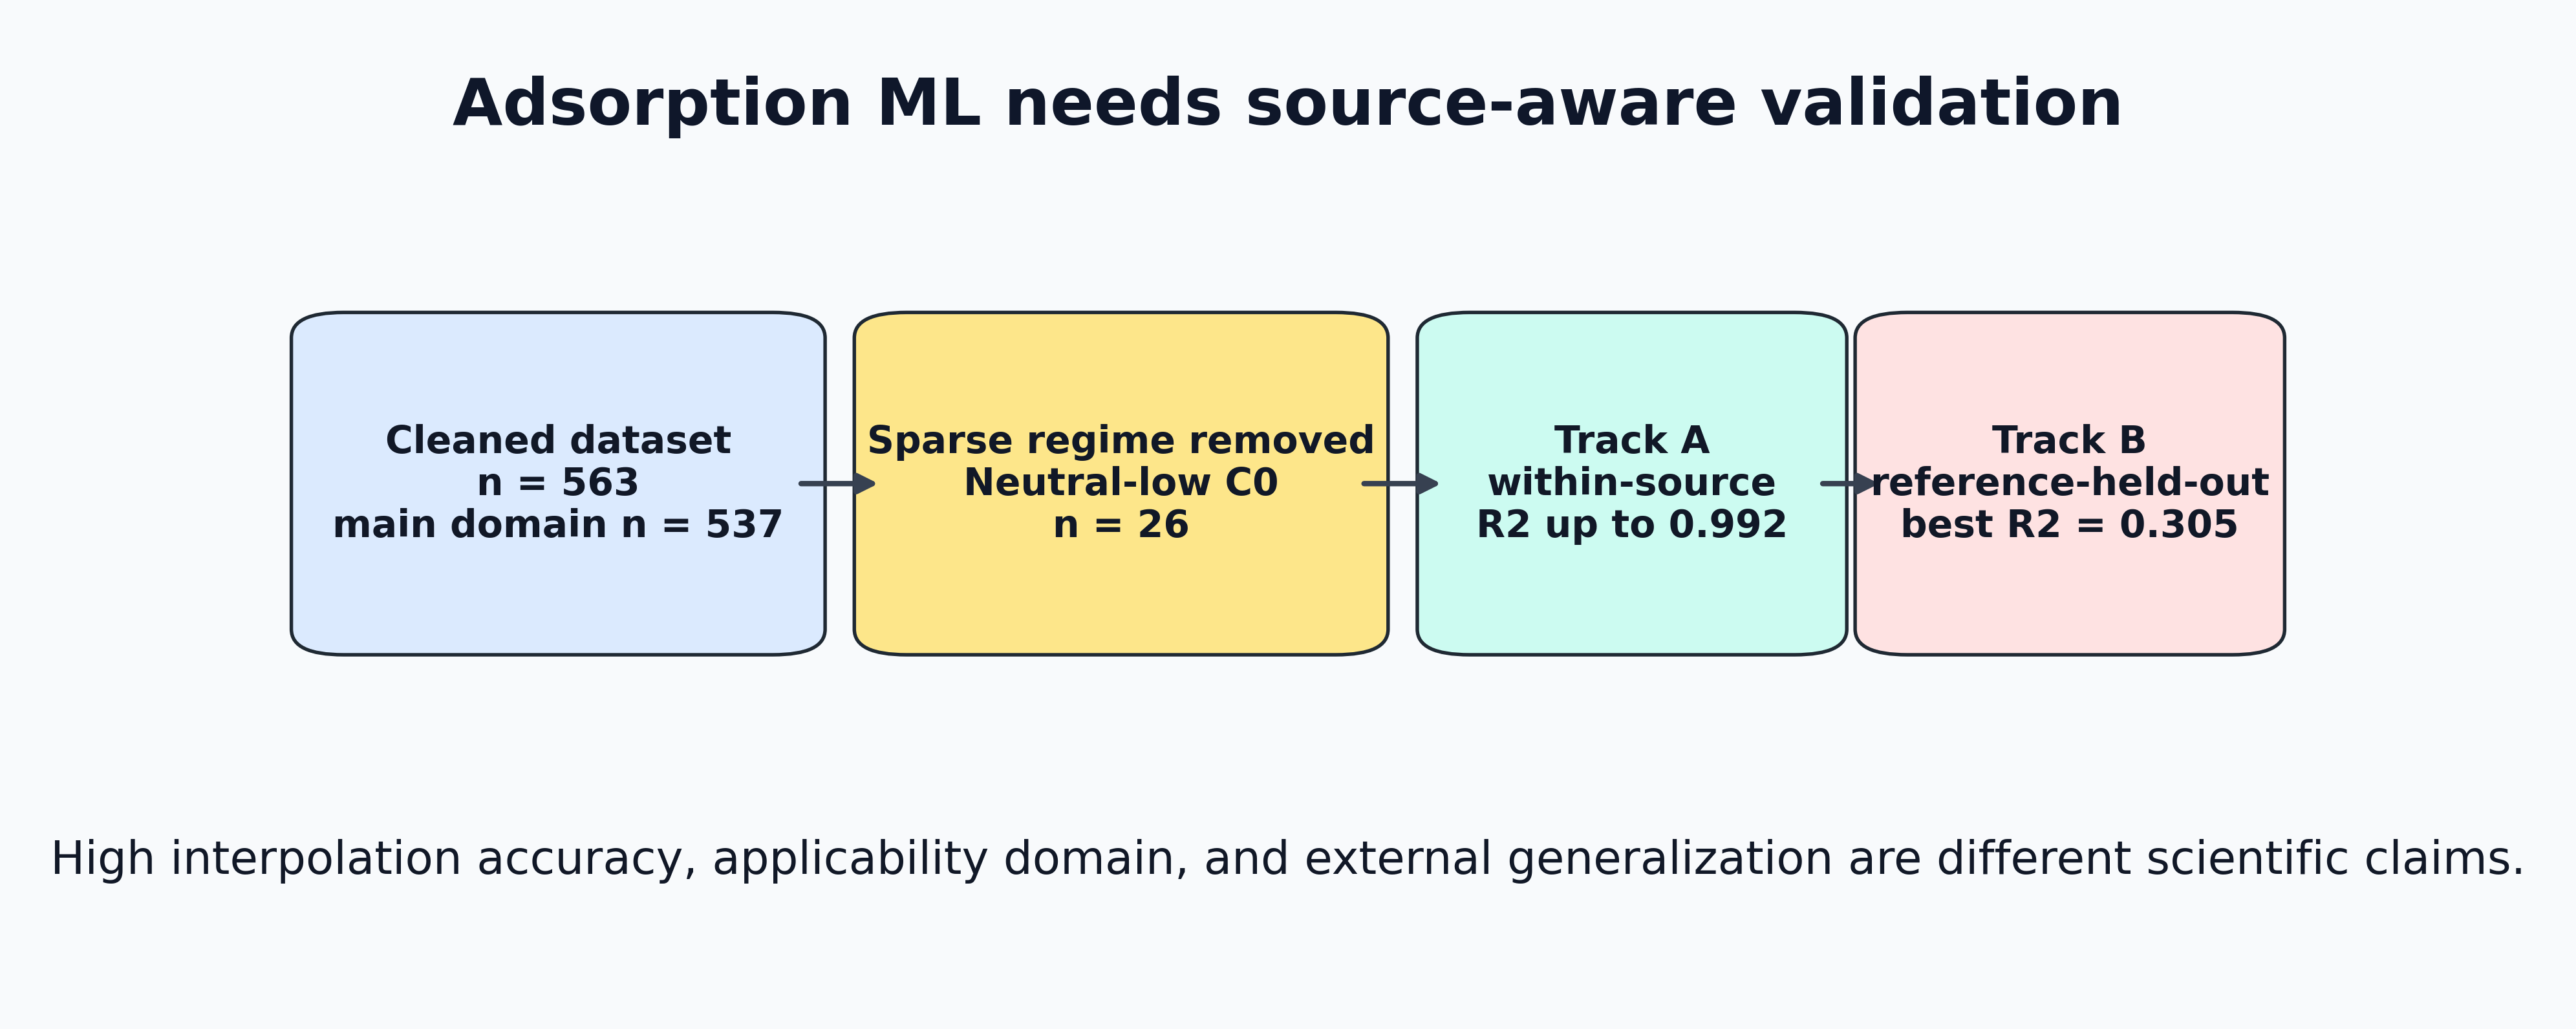
\includegraphics[width=\linewidth]{graphical_abstract.png}
\end{graphicalabstract}

\begin{highlights}
\item Source-specific adsorption models reached $R^2$ up to 0.992.
\item Sparse neutral-low-concentration cases were excluded from primary modeling.
\item Row-wise validation overstated source-transfer performance.
\item Reference-held-out screening reached $R^2 = 0.305$ in the main domain.
\item Capacity-inclusive and capacity-free models served distinct uses.
\end{highlights}

\begin{frontmatter}

\title{Source-aware machine learning for heavy-metal adsorption: distinguishing high-accuracy interpolation from cross-source generalization}

\author[inst1]{Yash Bisht\corref{cor1}}
\author[inst2]{Susmit Chitransh}
\cortext[cor1]{Corresponding author.}

\address[inst1]{Department of Mechanical and Industrial Engineering, Indian Institute of Technology Roorkee, Roorkee 247667, Uttarakhand, India}
\address[inst2]{Department of Chemical Engineering, University of Cape Town, Rondebosch 7700, Cape Town, South Africa}

\begin{abstract}
Machine learning is increasingly used to predict adsorption removal efficiency for water and wastewater treatment, but reported performance can depend strongly on feature definition, domain coverage, and validation design. This study develops a source-aware and leakage-aware framework for heavy-metal adsorption removal-efficiency prediction using a literature-compiled experimental dataset. The raw dataset contained 566 adsorption records; after deterministic numeric parsing and quality filtering, 563 valid records remained. Because the neutral/low-concentration regime contained only 26 observations, primary modeling was restricted to the remaining 537 records covering acidic/high-concentration, acidic/low-concentration, and neutral/high-concentration regimes. Four feature sets were evaluated to separate capacity-inclusive process-monitoring models from capacity-free pre-experiment screening models. Track A quantified source-specific interpolation through within-source cross-validation, where XGBoost reached $R^2$ values of 0.992, 0.974, and 0.960 for three major source groups. Track B evaluated broader generalization through repeated random row-wise, adsorbent-held-out, and reference-held-out splits. In the restricted primary domain, the full capacity-inclusive LightGBM model achieved $R^2 = 0.806$ under random row-wise validation. The best adsorbent-held-out result was obtained by a capacity-free numeric XGBoost model ($R^2 = 0.520$), and the best reference-held-out result was obtained by a capacity-free numeric ExtraTrees model ($R^2 = 0.305$). These results show that high adsorption-prediction accuracy is meaningful for in-source interpolation, but broader deployment requires explicit applicability-domain definition and source-held-out validation.
\end{abstract}

\begin{keyword}
adsorption \sep heavy metals \sep removal efficiency \sep machine learning \sep XGBoost \sep source-aware validation \sep wastewater treatment
\end{keyword}

\end{frontmatter}

\linenumbers

\section{Introduction}

Heavy-metal contamination remains a persistent challenge for water and wastewater treatment because metals such as Pb, Cd, Cr, Ni, Cu, As, Hg, and Zn are toxic, non-biodegradable, and prone to accumulation in environmental and biological systems. Adsorption is widely investigated for heavy-metal removal because it can operate under mild conditions, can be adapted to low-cost or waste-derived adsorbents, and can be optimized through pH, adsorbent dose, contact time, temperature, surface chemistry, and initial contaminant concentration. The expansion of experimental adsorption datasets has therefore encouraged the use of machine learning (ML) to predict removal efficiency and accelerate adsorbent screening.

Recent adsorption and environmental-remediation ML studies demonstrate that high predictive accuracy is possible. Hafsa et al. modeled heavy-metal adsorption efficiencies using multiple ML algorithms and reported $R^2$ values in the 0.96--0.99 range under ten-fold cross-validation, with experimental data supplemented by synthetic interpolation \cite{hafsa2020}. Lu et al. predicted heavy-metal removal by chitosan-based flocculants using random forests and reported $R^2 = 0.9354$, identifying solution pH and flocculant molecular weight as important drivers \cite{lu2022}. Wang et al. used interpretable ML for heavy-metal removal by biochar and reported XGBoost test performance near $R^2 = 0.99$, together with SHAP and partial-dependence analyses to relate removal efficiency to biochar and operating variables \cite{wang2024,lundberg2017}. Recent ensemble-learning work on biochar adsorption similarly reported strong XGBoost performance for heavy-metal adsorption efficiency prediction \cite{yaseen2025}. Within the scope of \textit{Journal of Environmental Chemical Engineering}, interpretable XGBoost modeling has also been applied to heavy-metal removal efficiency in electrokinetic remediation, demonstrating the journal relevance of transparent ML workflows for environmental treatment systems \cite{barkhordari2024}.

The central challenge is that high row-wise validation performance does not necessarily imply generalization to unseen laboratories, adsorbents, pollutant systems, or source studies. In ML-based science, data leakage and validation mismatch can produce overoptimistic estimates of deployable performance \cite{kapoor2023}. Environmental ML best-practice guidance similarly emphasizes careful data splitting, leakage management, randomness assessment, and evaluation design \cite{zhu2023}. These concerns are particularly important for adsorption datasets because different sources may use different adsorbent synthesis routes, contaminant species, concentration ranges, analytical protocols, and reporting conventions. A random row-wise split can place related observations from the same reference, adsorbent family, or operating campaign into both the training and test sets. Such a model may perform well, but the result primarily measures interpolation within a familiar experimental domain.

Feature definition can further blur the interpretation of reported accuracy. Adsorption capacity and removal efficiency are both derived from concentration changes in many batch adsorption experiments:

\begin{equation}
\mathrm{RE}(\%) = 100\frac{C_0-C_e}{C_0},
\end{equation}

\begin{equation}
q_e = \frac{(C_0-C_e)V}{m},
\end{equation}

where $C_0$ and $C_e$ are the initial and equilibrium concentrations, $V$ is the solution volume, and $m$ is the adsorbent mass. Capacity can therefore be useful for process monitoring after adsorption has been measured, but it should be treated cautiously in pre-experiment screening models where capacity is not yet available. Recent PFAS adsorption modeling has similarly shown that random-split performance can be much stronger than leave-one-compound-out performance, illustrating that interpolation and transfer to unseen chemical domains are distinct tasks \cite{patel2026}.

This study addresses these issues by developing a dual-track validation framework for heavy-metal adsorption removal-efficiency prediction. Track A evaluates source-specific interpolation and asks whether high $R^2$ values comparable to the adsorption-ML literature can be reproduced within individual source groups. Track B evaluates global generalization under random row-wise, adsorbent-held-out, and reference-held-out validation. The study further separates capacity-inclusive process-monitoring models from capacity-free screening models. The novelty is not simply a new regression model; rather, it is a source-aware reporting framework that clarifies when high $R^2$ is scientifically valid, when it is validation-dependent, and how adsorption ML studies should present performance for practical environmental-engineering use.

\section{Materials and methods}

\subsection{Dataset and target variable}

The dataset was compiled from reported heavy-metal adsorption experiments. Each record corresponds to one adsorption condition with a reported removal efficiency. The raw dataset contained 566 rows and 13 columns. After numeric parsing, missing-value filtering, and constraining removal efficiency to the physically meaningful range 0--100\%, 563 records remained. The cleaned dataset included 189 normalized source references, 219 adsorbents, and 16 normalized adsorbate classes. The primary modeling domain excluded the sparse neutral/low-concentration regime, leaving 537 records for model training and testing.

The target variable was removal efficiency, RE (\%). Input variables included adsorbent name, adsorbate identity, surface area, adsorption capacity, initial concentration, contact time, adsorbent dose, agitation speed, initial pH, temperature, and source reference. The source identifier, denoted \texttt{Ref\_group}, was used as a source-origin proxy because explicit laboratory-origin labels were not available for all records.

\subsection{Numeric cleaning and categorical normalization}

Literature-derived adsorption tables often contain nonuniform numeric formatting. Numeric entries were cleaned using deterministic rules: decimal commas were converted to decimal points, uncertainty and approximate symbols were removed, multiple values in one cell were reduced to the first numeric value, and nonnumeric text was parsed using regular expressions. Rows with missing values in required numeric variables were removed. Adsorbate names were normalized to reduce duplicates such as elemental and valence-state aliases. Adsorbent names were grouped into broad families, including carbon-based, mineral/oxide, polymer, biomass, and composite/other categories.

The cleaned data were assigned to four pH-concentration regimes using pH = 7 and the median initial concentration, $C_0 = 50$ ppm (Table~\ref{tab:regimes}). These regimes were not model targets; they were used to preserve chemically meaningful coverage during random splitting and to diagnose whether performance was dominated by a single operating region. The acidic regimes dominated the dataset, whereas the neutral/low-concentration regime contained only 26 observations. Because this regime was too small for stable split-wise evaluation, it was excluded from the primary ML domain and retained as an explicit out-of-domain limitation.

\begin{table}[htbp]
\centering
\caption{pH-concentration regime distribution in the cleaned dataset.}
\label{tab:regimes}
\small
\begin{tabular}{lrrrr}
\toprule
Regime & Count & Mean pH & Mean $C_0$ (ppm) & Mean RE (\%) \\
\midrule
Acidic\_HighC0 & 246 & 4.51 & 190.27 & 70.30 \\
Acidic\_LowC0 & 231 & 5.12 & 11.04 & 74.06 \\
Neutral\_HighC0 & 60 & 7.65 & 166.51 & 68.05 \\
Neutral\_LowC0 & 26 & 7.47 & 20.24 & 81.41 \\
\bottomrule
\end{tabular}
\parbox{0.95\linewidth}{\footnotesize Neutral\_LowC0 was excluded from primary modeling because it contained only 26 observations; the other three regimes formed the 537-record primary domain.}
\end{table}

\subsection{Feature sets}

Four feature sets were constructed to distinguish scientific use cases (Table~\ref{tab:features}). This separation is important because a model that includes adsorption capacity answers a different question from a model intended for pre-experiment adsorbent screening. The base experimental inputs were surface area, initial concentration, contact time, dose, agitation speed, initial pH, and temperature. The process-monitoring feature set additionally used adsorption capacity and capacity-derived terms, whereas the screening feature sets deliberately removed these terms.

\begin{table}[htbp]
\centering
\caption{Feature-set definitions used to separate process-monitoring and screening tasks.}
\label{tab:features}
\small
\begin{tabular}{>{\raggedright\arraybackslash}p{0.28\linewidth}>{\raggedright\arraybackslash}p{0.42\linewidth}>{\raggedright\arraybackslash}p{0.22\linewidth}}
\toprule
Feature set & Included information & Intended use \\
\midrule
Full capacity process model & Operating variables, surface area, adsorption capacity, capacity-derived ratios, ion descriptors, adsorbent family, and adsorbate identity & Descriptive or process-monitoring prediction \\
Screening-safe plus ion & Operating variables, surface area, engineered process variables, ion descriptors, and adsorbent family; excludes capacity terms & Pre-experiment screening with ion chemistry \\
Screening-safe plus adsorbate one-hot & Operating variables, surface area, engineered process variables, adsorbate identity, and adsorbent family; excludes capacity terms & Screening where pollutant identity is known \\
Screening-safe numeric-only & Operating variables, surface area, and engineered process variables; excludes capacity and adsorbate identity & Strict screening baseline \\
\bottomrule
\end{tabular}
\end{table}

Physics-inspired variables included site density, logarithmic contact time, mixing index, driving-force proxy, and acidity strength:

\begin{align}
\mathrm{Site\ Density} &= \frac{\mathrm{dose}\times \mathrm{surface\ area}}{C_0}, \\
\mathrm{LogTime} &= \log(1+\mathrm{contact\ time}), \\
\mathrm{Mixing\ Index} &= \mathrm{RPM}\times \mathrm{LogTime}, \\
\mathrm{Driving\ Force} &= \frac{C_0}{\mathrm{dose}}, \\
\mathrm{Acidity\ Strength} &= |\mathrm{pH}-7|.
\end{align}

Ion descriptors included charge, ionic radius, hydrated radius, ionic potential, and hydration ratio. These descriptors were used to reduce dependence on one-hot pollutant labels and to encode basic aqueous-ion chemistry.

The full model therefore used the following ML inputs: seven operating/material numeric variables; adsorption capacity, capacity-loading ratio, and thermo-capacity; five engineered process descriptors; six ion descriptors; normalized adsorbate identity; and broad adsorbent family. The capacity-free models retained the operating/material variables and engineered descriptors but removed adsorption capacity, capacity-loading ratio, and thermo-capacity. Among the capacity-free models, one retained ion descriptors, one used normalized adsorbate identity, and the strictest model used numeric variables only.

\subsection{Machine-learning models}

XGBoost was selected as the primary model because gradient-boosted trees are effective for nonlinear tabular datasets and are widely used in adsorption ML studies \cite{chen2016,friedman2001}. LightGBM was included as an additional gradient-boosting comparator because preliminary model development indicated similar row-wise interpolation performance. Extremely randomized trees (ExtraTrees) were included as a comparator ensemble model because random forest-style tree ensembles provide robust nonlinear baselines for tabular prediction \cite{breiman2001,geurts2006}. A mean dummy regressor was included to quantify improvement beyond a no-skill baseline.

Categorical variables were one-hot encoded with unknown-category handling, while numerical variables were passed directly to the tree models. XGBoost used 140 estimators, learning rate 0.05, maximum depth 4, subsample 0.85, column subsample 0.85, $\ell_1$ regularization 0.1, and $\ell_2$ regularization 1.0. LightGBM used 300 estimators, learning rate 0.05, maximum depth 5, 31 leaves, minimum child samples 15, subsample 0.85, column subsample 0.85, $\ell_1$ regularization 0.1, and $\ell_2$ regularization 0.5. ExtraTrees used 120 estimators, maximum depth 10, and minimum leaf size 2. Predictions were clipped to the physically meaningful RE range of 0--100\% before metric calculation.

\subsection{Validation design}

Two validation tracks were used (Fig.~\ref{fig:workflow}). Track A evaluated source-specific interpolation. For each reference with at least 20 records and sufficient target variability, source-specific 5-fold cross-validation was performed using shuffled folds with a fixed random seed. This tests whether high $R^2$ values are achievable within a known experimental source, which is similar to the validation setting of many high-performance adsorption ML studies.

Track B evaluated global generalization using three validation protocols within the restricted primary domain. The random row-wise split used an 80/20 train-test split stratified by the three retained pH-concentration regimes, so each split retained acidic/high-$C_0$, acidic/low-$C_0$, and neutral/high-$C_0$ observations. The adsorbent-held-out split used group splitting so that exact adsorbent names in the test set were absent from the training set. This split should be interpreted as an applicability-domain stress test for new adsorbent identities with known descriptors, not as a claim that the model can predict an entirely undescribed material from its name. The reference-held-out split used group splitting so that entire references/sources were absent from the training set. Each Track B protocol was repeated over five random seeds. Metrics included $R^2$, root mean squared error (RMSE), mean absolute error (MAE), and prediction bias.

\begin{figure}[htbp]
\centering
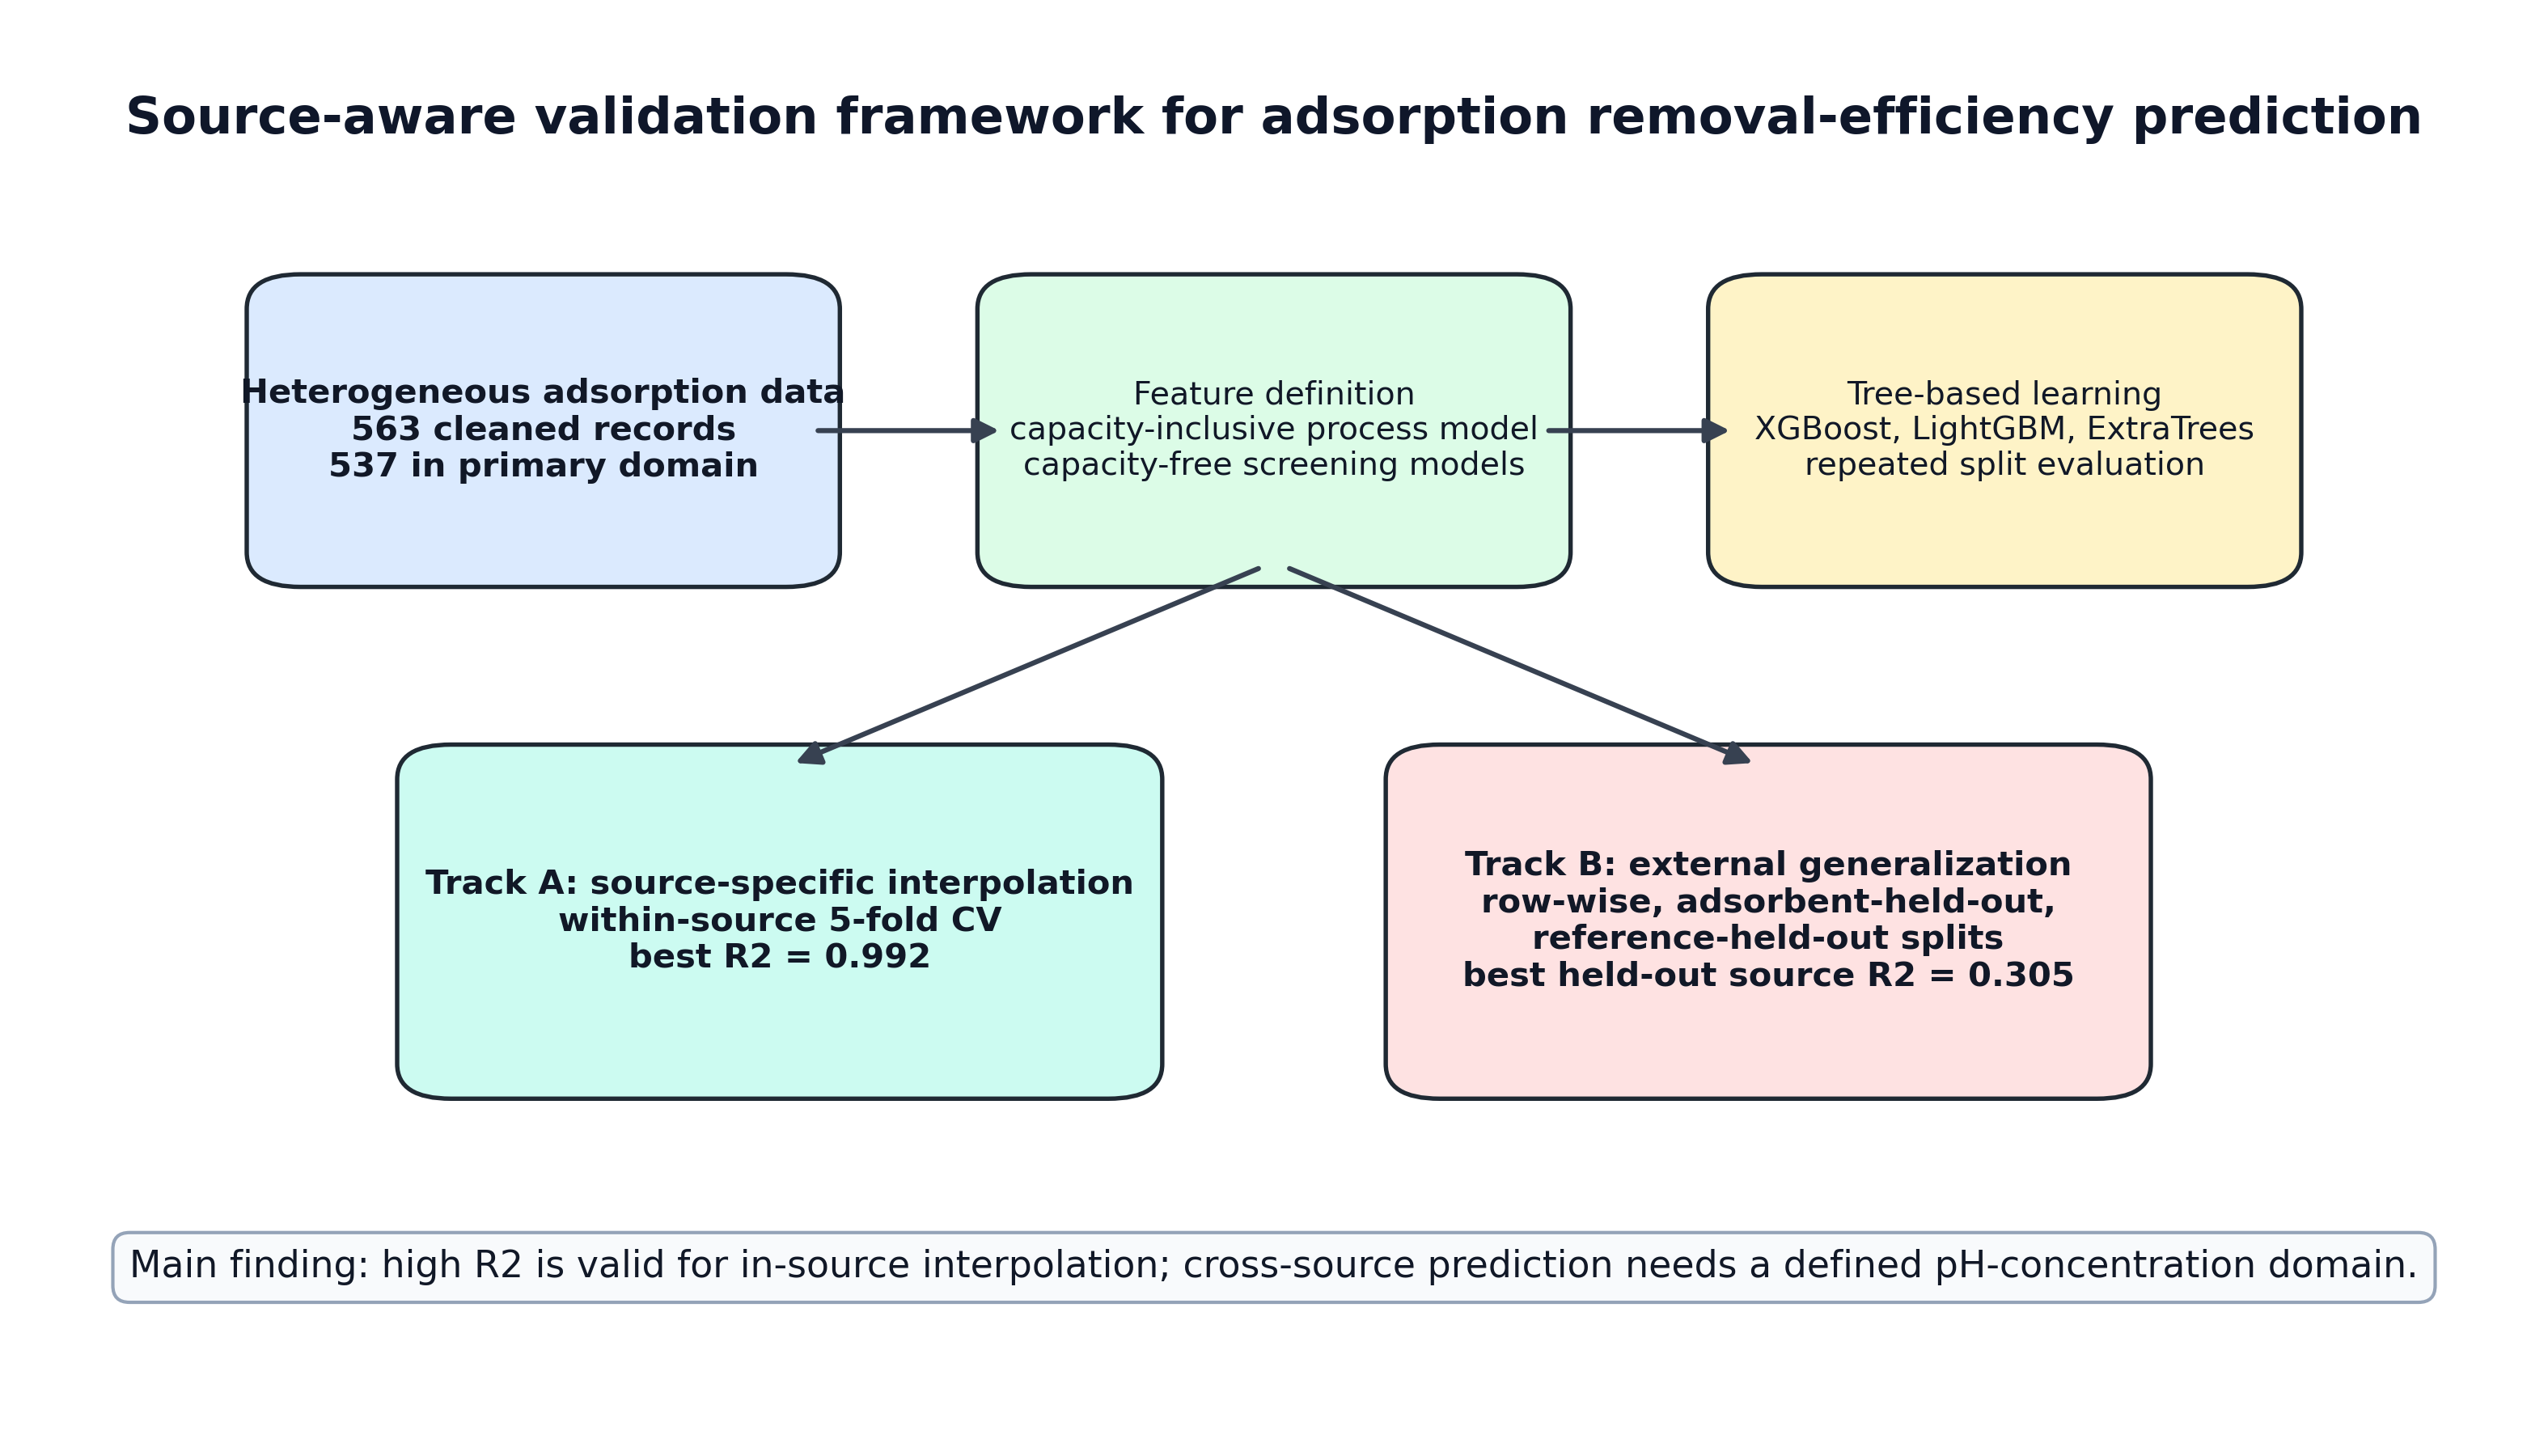
\includegraphics[width=0.95\linewidth]{figure_1_workflow.png}
\caption{Workflow of the proposed source-aware adsorption-ML validation framework. Track A measures source-specific interpolation, whereas Track B measures progressively stricter global generalization.}
\label{fig:workflow}
\end{figure}

\section{Results}

\subsection{Source-specific models reproduced high adsorption-prediction accuracy}

Track A showed that high removal-efficiency prediction accuracy is achievable when models are trained and evaluated within individual source groups. The full capacity process model achieved $R^2 = 0.9916$ for the source group Shen et al. (2017b), $R^2 = 0.9735$ for Gao et al. (2019), and $R^2 = 0.9601$ for Zama et al. (2017). These results are in the range commonly reported in adsorption ML studies under row-wise or within-domain validation \cite{hafsa2020,wang2024,lu2022}.

\begin{table}[htbp]
\centering
\caption{Track A source-specific 5-fold cross-validation results for the full capacity process model.}
\label{tab:tracka}
\begin{tabular}{lrrrr}
\toprule
Source group & Rows & $R^2$ & RMSE & MAE \\
\midrule
Shen et al. (2017b) & 65 & 0.9916 & 3.20 & 2.33 \\
Gao et al. (2019) & 48 & 0.9735 & 2.97 & 2.14 \\
Zama et al. (2017) & 91 & 0.9601 & 7.84 & 3.56 \\
Cui et al. (2016a) & 24 & 0.8936 & 6.65 & 4.56 \\
\bottomrule
\end{tabular}
\end{table}

\begin{figure}[htbp]
\centering
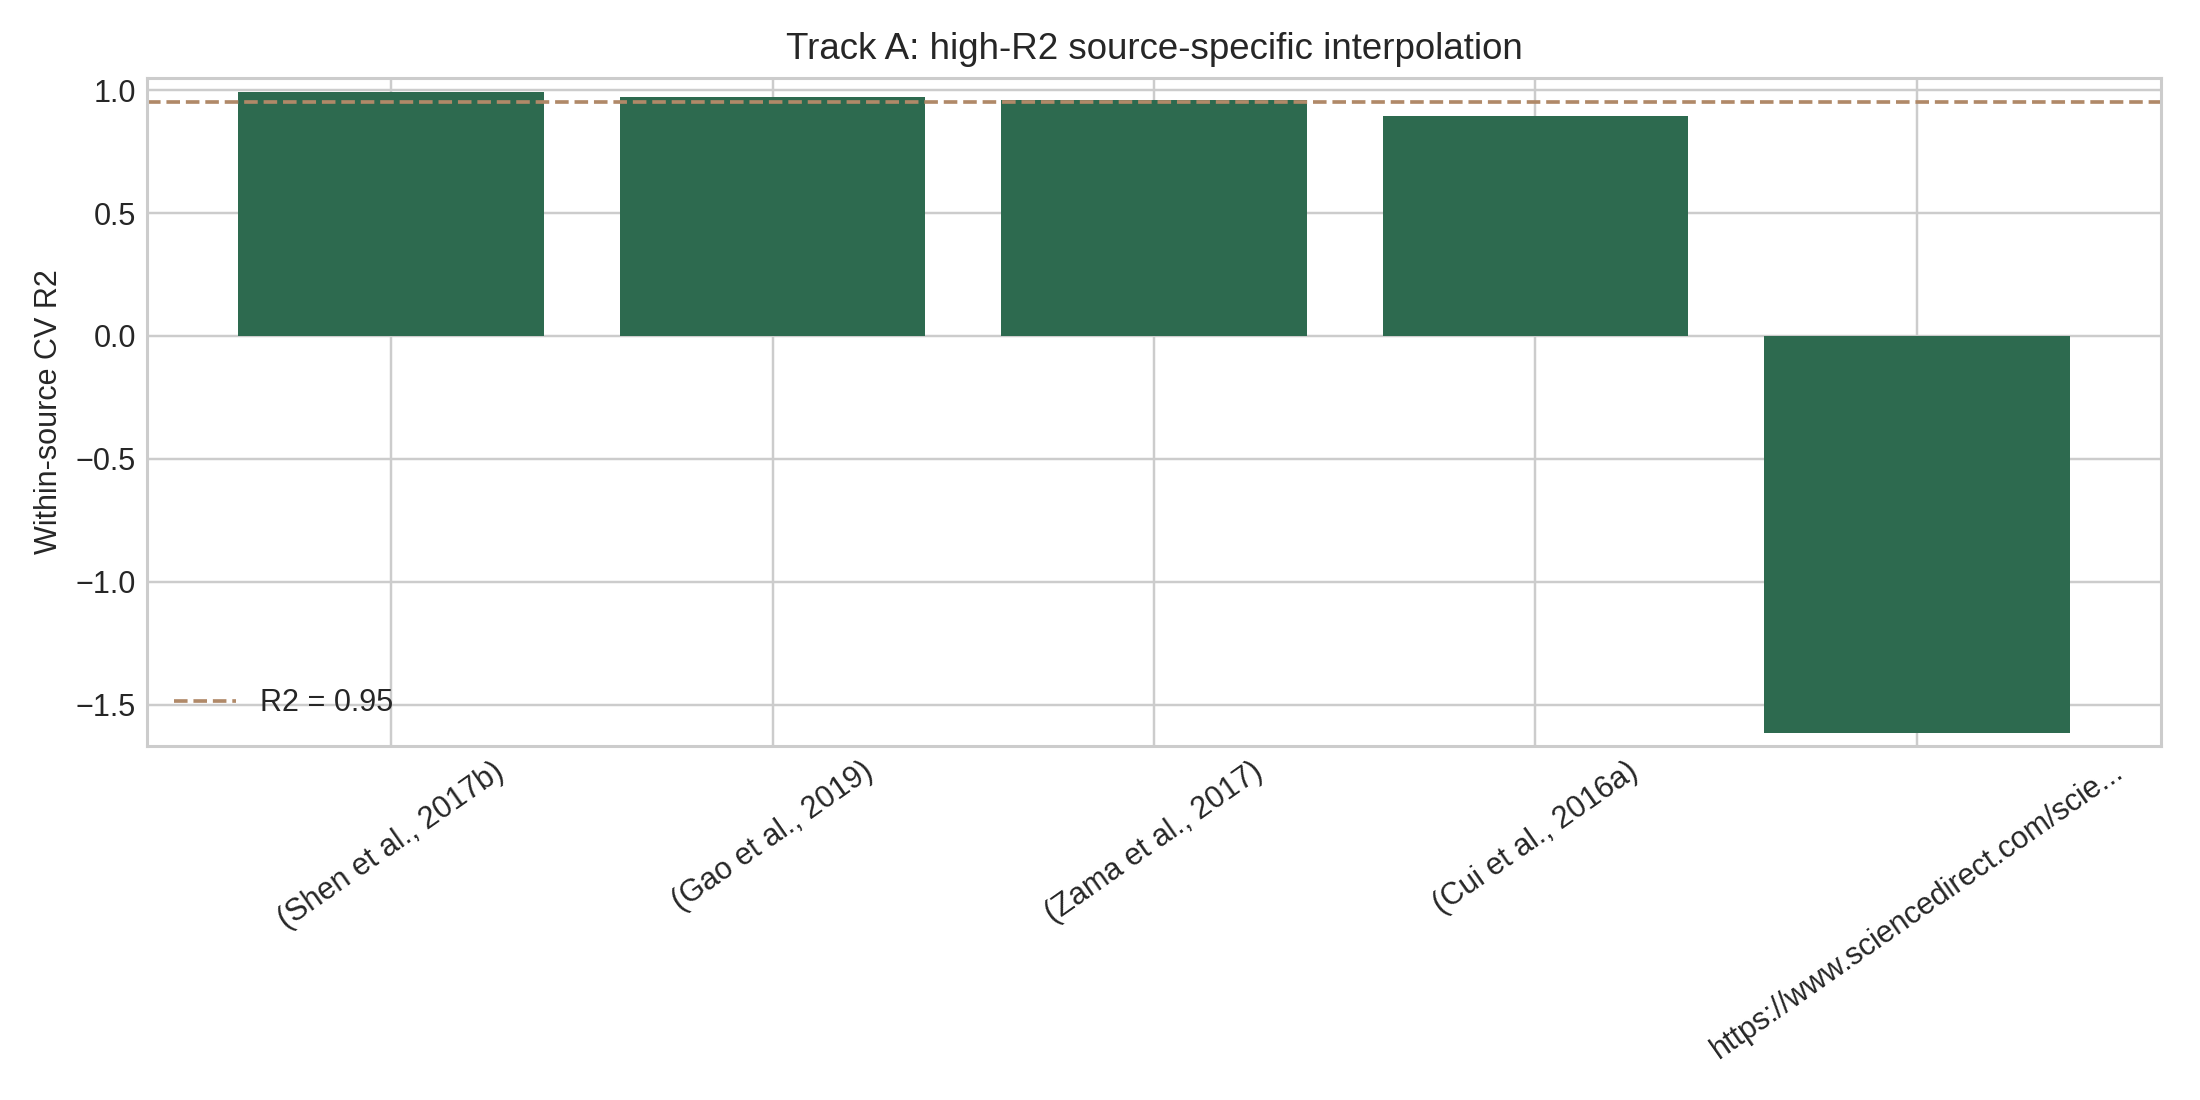
\includegraphics[width=0.95\linewidth]{track_a_within_source_r2.png}
\caption{Track A source-specific interpolation performance. Several individual source-group models achieved $R^2$ values near or above 0.95, while other source groups remained more difficult.}
\label{fig:tracka}
\end{figure}

Capacity-free source-specific models also performed well in selected source groups. For example, the source-specific model for Zama et al. (2017) achieved $R^2 = 0.9250$ using the screening-safe ion feature set, while Shen et al. (2017b) achieved $R^2$ values above 0.91 using capacity-free screening feature sets. This indicates that high source-specific performance is not solely a capacity-inclusion artifact, although capacity-inclusive models generally gave the strongest interpolation performance.

\subsection{Random row-wise validation produced moderate-to-good global performance}

Under repeated random row-wise splits in the restricted primary domain, the full capacity process model achieved $R^2 = 0.8064$ and RMSE = 12.94 with LightGBM, while the corresponding XGBoost model achieved $R^2 = 0.7985$ and RMSE = 13.22. The screening-safe plus adsorbate one-hot XGBoost model achieved $R^2 = 0.7283$ and RMSE = 15.29, while the screening-safe plus ion XGBoost model achieved $R^2 = 0.7265$ and RMSE = 15.34. Thus, even without adsorption capacity, the model retained useful predictive ability under in-dataset interpolation (Table~\ref{tab:trackb_random}).

\begin{table}[htbp]
\centering
\caption{Restricted-domain random row/regime split performance after excluding the sparse neutral/low-$C_0$ regime. Values are means over five repeated splits.}
\label{tab:trackb_random}
\begin{tabular}{lrrr}
\toprule
Feature/model & $R^2$ & RMSE & MAE \\
\midrule
Full capacity LightGBM & 0.8064 & 12.94 & 8.08 \\
Full capacity XGBoost & 0.7985 & 13.22 & 8.44 \\
Full capacity ExtraTrees & 0.7730 & 14.02 & 9.02 \\
Screening-safe plus adsorbate XGBoost & 0.7283 & 15.29 & 10.84 \\
Screening-safe plus ion XGBoost & 0.7265 & 15.34 & 10.88 \\
\bottomrule
\end{tabular}
\end{table}

These results support the use of ML for in-domain adsorption prediction. They also explain the strong preliminary LightGBM results obtained during model development: earlier LightGBM runs used the same type of random/regime-stratified split and included capacity-related predictors, giving global $R^2$ values around 0.84--0.86 depending on the exact feature set and domain filter. Those values are valid row-wise interpolation results, but they are not evidence of source-held-out generalization. Random row-wise validation alone is therefore not sufficient evidence for deployment on unseen sources.

\subsection{Generalization weakened under adsorbent- and reference-held-out validation}

The validation protocol strongly affected performance. When entire adsorbents were held out, the best result was obtained by the screening-safe numeric-only XGBoost model, with $R^2 = 0.5199$ and RMSE = 19.61. The corresponding LightGBM screening model achieved $R^2 = 0.5002$, while the full capacity XGBoost process model achieved $R^2 = 0.4385$. This indicates moderate but imperfect transfer to unseen adsorbent names when their measured descriptors are available. It should not be interpreted as prediction for a completely undescribed adsorbent.

Reference-held-out validation was more difficult than row-wise validation but improved markedly after removing the sparse neutral/low-$C_0$ regime. The best reference-held-out result was obtained by the screening-safe numeric-only ExtraTrees model, with $R^2 = 0.3054$ and RMSE = 23.54. The full capacity LightGBM model achieved $R^2 = 0.2820$, while the full capacity XGBoost model achieved $R^2 = 0.1678$. These results remain below row-wise performance, but they show that defining a better-covered applicability domain produces more meaningful external-source validation.

\begin{table}[htbp]
\centering
\caption{Restricted-domain Track B generalization performance after excluding the sparse neutral/low-$C_0$ regime. Values are means over five repeated splits.}
\label{tab:trackb_group}
\small
\begin{tabular}{>{\raggedright\arraybackslash}p{0.27\linewidth}>{\raggedright\arraybackslash}p{0.35\linewidth}rrr}
\toprule
Validation & Feature/model & $R^2$ & RMSE & MAE \\
\midrule
Holdout adsorbent & Screening-safe numeric-only XGBoost & 0.5199 & 19.61 & 15.15 \\
Holdout adsorbent & Screening-safe numeric-only LightGBM & 0.5002 & 20.10 & 15.19 \\
Holdout adsorbent & Full capacity XGBoost & 0.4385 & 20.76 & 13.94 \\
Holdout reference/source & Screening-safe numeric-only ExtraTrees & 0.3054 & 23.54 & 18.67 \\
Holdout reference/source & Full capacity LightGBM & 0.2820 & 23.78 & 18.67 \\
Holdout reference/source & Full capacity XGBoost & 0.1678 & 25.66 & 19.53 \\
\bottomrule
\end{tabular}
\end{table}

\begin{figure}[htbp]
\centering
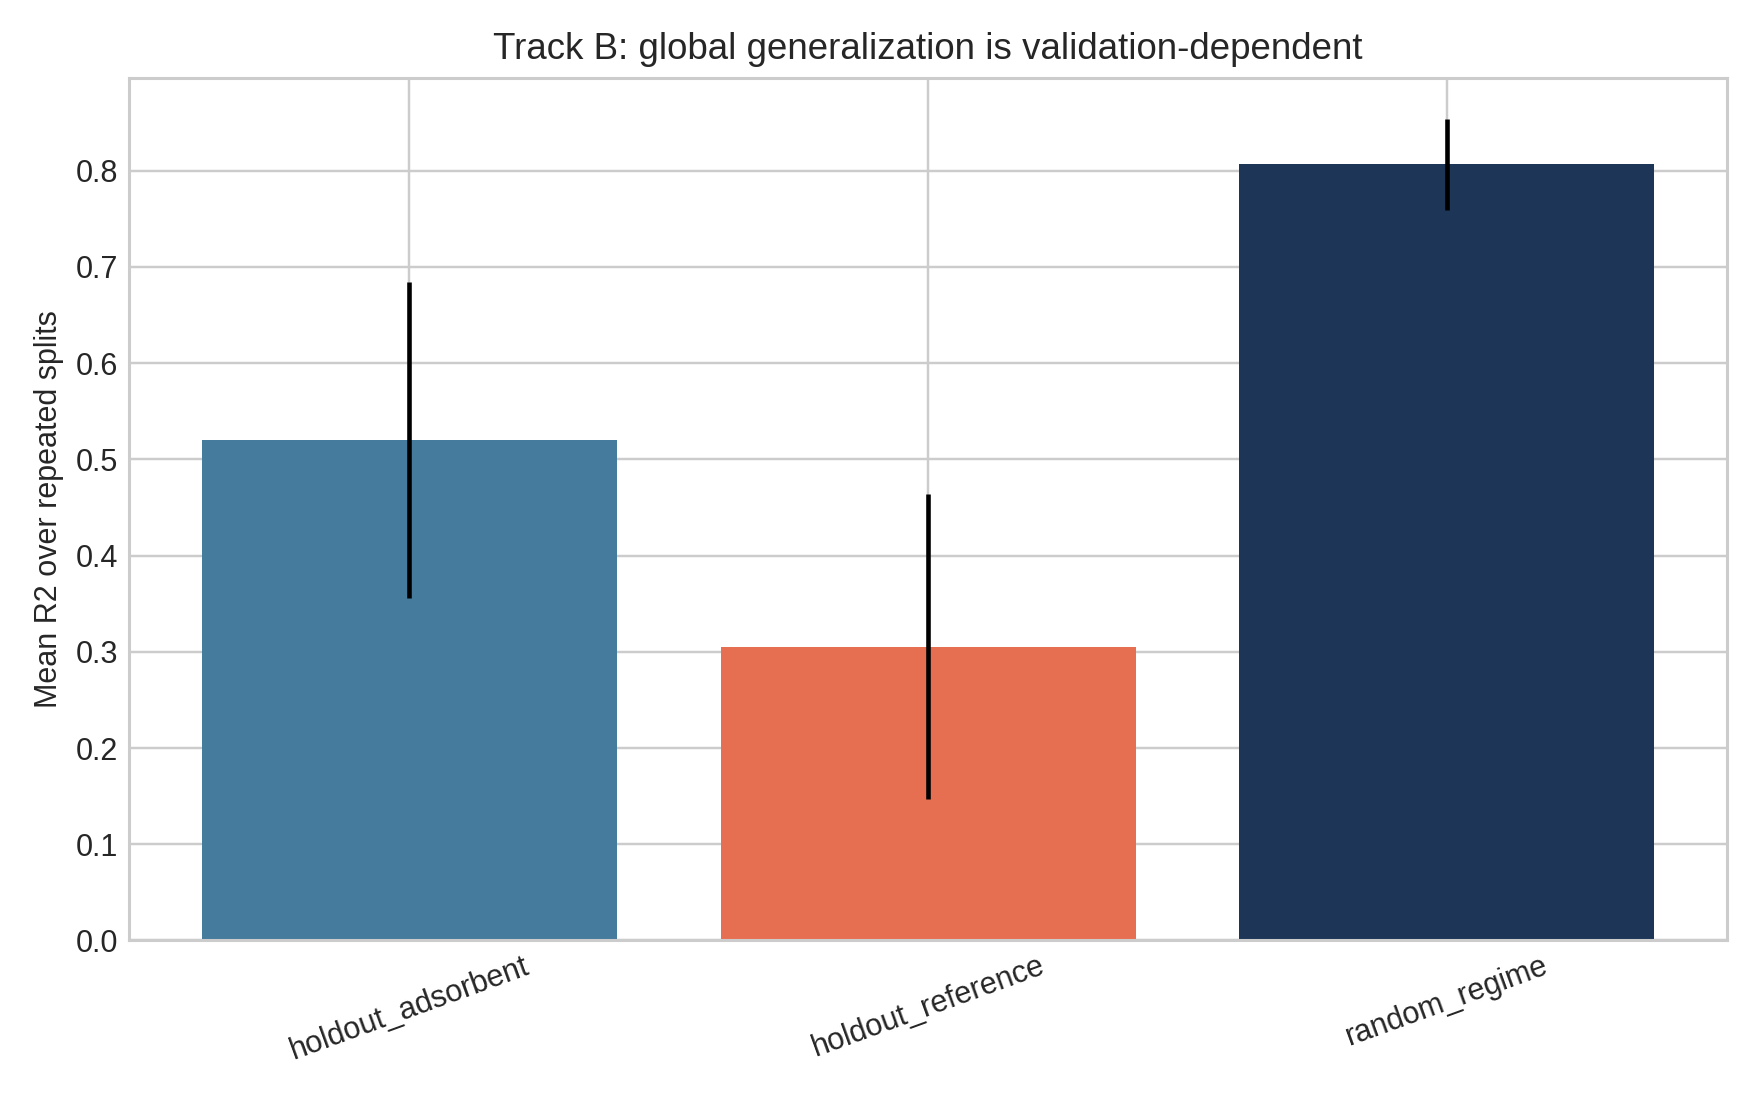
\includegraphics[width=0.85\linewidth]{track_b_global_split_r2.png}
\caption{Track B validation comparison. Row-wise validation, adsorbent-held-out validation, and reference-held-out validation represent increasingly strict generalization tasks.}
\label{fig:trackb}
\end{figure}

These results show that removal-efficiency prediction is strongly source-dependent. The same data and model family can produce high $R^2$ under source-specific interpolation, moderate-to-good $R^2$ under random global validation, and lower but still informative $R^2$ under source-held-out validation when the applicability domain is restricted to sufficiently represented pH-concentration regimes.

\subsection{Capacity-inclusive and capacity-free models answered different questions}

The full capacity process model performed best for random row-wise validation and several source-specific models. This is expected because adsorption capacity carries strong information about adsorption performance. However, capacity can be outcome-adjacent to RE and may not be available before an experiment. Therefore, capacity-inclusive models should be framed as process-monitoring or descriptive models. Capacity-free models are more appropriate for pre-experiment screening and adsorbent-design guidance. In the restricted-domain adsorbent-held-out and reference-held-out tests, capacity-free numeric models were competitive or superior, suggesting that simpler descriptor sets can be more robust when transferring across material identities or source studies.

\section{Discussion}

\subsection{Why near-0.95 $R^2$ is achievable but validation-dependent}

The Track A results explain why many adsorption ML studies report $R^2$ values near or above 0.95. Within a single source, adsorbent family, pollutant system, or experimental protocol, the response surface can be learned accurately by tree-based models. In this setting, high $R^2$ is scientifically plausible and not automatically invalid. The present results reproduce that behavior, with source-specific $R^2$ values of 0.960--0.992 for three major source groups.

However, Track B shows that this performance should not be interpreted as universal adsorption prediction. When sources are held out, the model must transfer across experimental protocols, adsorbent synthesis methods, pollutant distributions, concentration ranges, and reporting conventions. Under that validation setting, performance fell below row-wise performance even after excluding the sparse neutral/low-$C_0$ regime. The result is consistent with recent adsorption-related work showing that random-split performance can be substantially higher than leave-compound-out performance \cite{patel2026}.

\subsection{Relation to existing adsorption ML literature}

The proposed framework complements rather than contradicts previous high-accuracy adsorption ML studies. Hafsa et al. demonstrated that tree-based algorithms can achieve high removal-efficiency prediction accuracy for heavy-metal adsorption datasets under repeated cross-validation \cite{hafsa2020}. Wang et al. showed that XGBoost, SHAP, and partial-dependence analyses can identify interpretable drivers of heavy-metal removal by biochar \cite{wang2024}. Lu et al. showed that random forests can predict heavy-metal removal by chitosan-based flocculants with $R^2$ above 0.93 \cite{lu2022}. Barkhordari et al. further demonstrated that interpretable XGBoost models are relevant to JECE's environmental-remediation scope by predicting heavy-metal removal efficiency in electrokinetic remediation \cite{barkhordari2024}. These studies establish that ML is useful for environmental treatment modeling.

The present study adds a validation-layer contribution: adsorption ML workflows should explicitly state whether they are predicting within a known source or generalizing to unseen sources. This distinction is critical because high row-wise $R^2$ can be overoptimistic when the deployment target is a new laboratory, adsorbent synthesis route, pollutant matrix, or literature source. The broader ML literature has identified leakage and validation mismatch as major reproducibility risks \cite{kapoor2023,zhu2023}, and adsorption datasets have several mechanisms by which such mismatch can occur.

\subsection{Practical implications for adsorption model deployment}

For practical adsorption screening, a single universal RE model should be used cautiously. A more defensible workflow is to define the pH-concentration applicability domain before modeling, exclude or separately model poorly represented regimes, use source-specific or laboratory-calibrated models for high-accuracy optimization within a known experimental system, use capacity-free screening models for preliminary adsorbent and operating-condition selection, and report source-held-out validation when predictions are intended for new adsorbents, pollutants, laboratories, or literature domains. This framing allows high-$R^2$ models to remain useful without overstating their generality.

\subsection{Limitations and future work}

This study has four main limitations. First, the dataset does not contain explicit laboratory-origin labels for all records; bibliographic reference was therefore used as a source proxy. Future work should annotate records as in-house, external-laboratory, or literature-derived and repeat validation with leave-laboratory-out splits. Second, the ion descriptor table should be expanded with fully cited descriptors such as electronegativity, hydration energy, softness/hardness, and likely aqueous speciation. Third, important adsorbent descriptors such as pH$_\mathrm{pzc}$, pore volume, pore size, zeta potential, FTIR-derived functional groups, and cation-exchange capacity are incomplete in the present dataset. Fourth, the neutral/low-concentration regime contained only 26 observations and was excluded from primary modeling; predictions in that regime should therefore be treated as outside the present applicability domain until more data are available. These limitations define clear routes for improving external predictive performance while preserving the source-aware validation principle.

\section{Conclusions}

This study developed a source-aware and leakage-aware framework for adsorption removal-efficiency prediction. High $R^2$ values were achievable within individual adsorption sources, with source-specific XGBoost models reaching $R^2$ up to 0.992. Because the neutral/low-concentration regime contained only 26 observations, primary global modeling excluded that sparse regime and used a 537-record restricted domain. Within this domain, random row-wise validation reached $R^2 = 0.806$ for the full capacity LightGBM process model, adsorbent-held-out validation reached $R^2 = 0.520$ for the capacity-free numeric XGBoost screening model, and reference-held-out validation reached $R^2 = 0.305$ for the capacity-free numeric ExtraTrees screening model. These findings show that high-accuracy interpolation, applicability-domain definition, and cross-source generalization are different scientific tasks. Future adsorption ML studies should report all three, separate capacity-inclusive process-monitoring models from capacity-free screening models, and include source- or laboratory-held-out validation when deployment beyond the training source is claimed.

\section*{CRediT authorship contribution statement}

Yash Bisht: Conceptualization, Methodology, Software, Formal analysis, Visualization, Writing -- original draft. Susmit Chitransh: Data curation, Investigation, Validation, Writing -- review and editing.

\section*{Declaration of competing interest}

The authors declare that they have no known competing financial interests or personal relationships that could have appeared to influence the work reported in this paper.

\section*{Funding}

This research did not receive any specific grant from funding agencies in the public, commercial, or not-for-profit sectors.

\section*{Data availability}

The curated dataset, analysis scripts, and generated benchmark outputs are available from the corresponding author upon reasonable request and will be deposited in a public repository before final publication.

\section*{Declaration of generative AI and AI-assisted technologies in the manuscript preparation process}

During the preparation of this work, the authors used OpenAI's Codex to assist with code organization, LaTeX formatting, and language polishing. After using this tool, the authors reviewed and edited the content as needed and take full responsibility for the content of the manuscript.

\section*{Acknowledgements}

The authors acknowledge the institutional support of the Indian Institute of Technology Roorkee and the University of Cape Town.

\begin{thebibliography}{99}

\bibitem{hafsa2020}
N. Hafsa, S. Rushd, M. Al-Yaari, M. Rahman, A generalized method for modeling the adsorption of heavy metals with machine learning algorithms, Water 12 (2020) 3490. \url{https://doi.org/10.3390/w12123490}.

\bibitem{lu2022}
C. Lu, Z. Xu, B. Dong, Y. Zhang, M. Wang, Y. Zeng, C. Zhang, Machine learning for the prediction of heavy metal removal by chitosan-based flocculants, Carbohydrate Polymers 285 (2022) 119240. \url{https://doi.org/10.1016/j.carbpol.2022.119240}.

\bibitem{wang2024}
C. Wang, Y. Zhao, Y. Gao, H. Chen, X. Li, B. Zhou, D. Fan, Z. Fang, J. Liu, Interpretable machine learning for predicting heavy metal removal and optimizing biochar characteristics, Journal of Water Process Engineering 68 (2024) 106484. \url{https://doi.org/10.1016/j.jwpe.2024.106484}.

\bibitem{yaseen2025}
Z.M. Yaseen, F.L. Alhalimi, Heavy metal adsorption efficiency prediction using biochar properties: a comparative analysis for ensemble machine learning models, Scientific Reports 15 (2025). \url{https://doi.org/10.1038/s41598-025-96271-5}.

\bibitem{barkhordari2024}
M.S. Barkhordari, N. Zhou, K. Li, C. Qi, Interpretable machine learning for predicting heavy metal removal efficiency in electrokinetic soil remediation, Journal of Environmental Chemical Engineering 12 (2024) 114330. \url{https://doi.org/10.1016/j.jece.2024.114330}.

\bibitem{lundberg2017}
S.M. Lundberg, S.-I. Lee, A unified approach to interpreting model predictions, in: Advances in Neural Information Processing Systems 30, 2017, pp. 4765--4774.

\bibitem{kapoor2023}
S. Kapoor, A. Narayanan, Leakage and the reproducibility crisis in machine-learning-based science, Patterns 4 (2023) 100804. \url{https://doi.org/10.1016/j.patter.2023.100804}.

\bibitem{zhu2023}
J.-J. Zhu, M. Yang, Z.J. Ren, Machine learning in environmental research: Common pitfalls and best practices, Environmental Science \& Technology 57 (2023) 17671--17689. \url{https://doi.org/10.1021/acs.est.3c00026}.

\bibitem{patel2026}
H.V. Patel, J. Green, H. Park, S. Luster-Teasley Pass, R. Zhao, A hybrid response surface methodology and machine learning framework for quantifying effects of physicochemical parameters on PFAS distribution, ACS ES\&T Water (2026) Advance online publication. \url{https://doi.org/10.1021/acsestwater.5c01162}.

\bibitem{chen2016}
T. Chen, C. Guestrin, XGBoost: A scalable tree boosting system, in: Proceedings of the 22nd ACM SIGKDD International Conference on Knowledge Discovery and Data Mining, ACM, San Francisco, CA, USA, 2016, pp. 785--794. \url{https://doi.org/10.1145/2939672.2939785}.

\bibitem{friedman2001}
J.H. Friedman, Greedy function approximation: A gradient boosting machine, Annals of Statistics 29 (2001) 1189--1232. \url{https://doi.org/10.1214/aos/1013203451}.

\bibitem{breiman2001}
L. Breiman, Random forests, Machine Learning 45 (2001) 5--32. \url{https://doi.org/10.1023/A:1010933404324}.

\bibitem{geurts2006}
P. Geurts, D. Ernst, L. Wehenkel, Extremely randomized trees, Machine Learning 63 (2006) 3--42. \url{https://doi.org/10.1007/s10994-006-6226-1}.

\end{thebibliography}

\end{document}
